% vim: spelllang=fr

\documentclass[../main.tex]{subfiles}
\graphicspath{{\subfix{../Figures/Chap1/}}}
\begin{document}

\begin{itshape}
Ce premier chapitre introduit les cyclones tropicaux (TC), de la simple définition jusqu'à la formulation de la question scientifique présentée dans cette thèse, en introduisant tous les concepts intermédiaires nécessaires.
\end{itshape}

\minitoc
%----------------------------------------------------------------------------
\section{Introduction aux cyclones tropicaux}

\subsection{Qu'est-ce qu'un cyclone tropical}\label{sec:quest_ce_qu_un_cyclone}

Du grec \textit{κύκλος}, nom commun désignant un cercle, ou plus généralement toute chose circulaire ou ronde, le terme cyclone, dans un contexte météorologique, fait référence au type de circulation atmosphérique dans lequel l'air se trouve en rotation atour d'un centre de basse pression. Sous cette définition, le terme de cyclone désigne une grande quantité d'objets aux caractéristiques très diverses et prenant place à différentes échelles spatiales et temporelles. Ainsi, à la
méso-échelle, ou échelle moyenne, caractérisée par des distances entre \SI{10}{\kilo\metre} et \SI{100}{\kilo\metre}, on peut par exemple citer les mésocyclones, vortex d'air ascendant et convergeant, mesurant généralement moins de \SI{10}{\kilo\metre} de diamètre et observés dans les systèmes météorologiques convectifs, comme notamment les orages super-cellulaires. De l'autre côté du spectre, à l'échelle synoptique, c'est à dire à l'échelle traitant des distances de l'ordre du millier de kilomètres et sur des
temps caractéristiques de quelques jours, les plus grands objets météorologiques dépressionnaires pouvant être qualifiés de cyclones sont sans
nulle doute les vortex polaires ; de larges dépressions d'altitude situées près des pôles géographiques et dans lesquelles de l'air froid est en rotation. Malgré ces différences apparentes, tous les cyclones possèdent néanmoins des caractéristiques communes. Ainsi, le centre du cyclone est toujours l'endroit où la pression atmosphérique est la plus faible, et la circulation de l'air autour du centre est assurée à minima par l'équilibre entre la force induite par le gradient de pression radial d'une part, et la somme
de la force centrifuge ainsi que la force de Coriolis d'autre part -- équilibre qualifié de cyclostrophique, ou équilibre du vent gradient. La force de Coriolis, force inertielle causée par la rotation de la Terre, est également la raison pour laquelle les cyclones tournent dans le sens contraire des aiguilles d'une montre dans l'hémisphère nord, et inversement dans l'hémisphère sud.

Les cyclones tropicaux -- que l'on abrègera ensuite par l'acronyme TC, selon l'appellation anglaise \textit{Tropical Cyclone} -- sont donc des phénomènes tourbillonnaires pouvant atteindre plusieurs centaines de kilomètres, les plaçant ainsi à la lisière entre la mésoéchelle et l'échelle synoptique. Ces objets prennent naissance, comme leur nom l'indique, dans la ceinture tropicale, définie comme la zone située entre le Tropique du Cancer dans l'hémisphère nord et le Tropique du Capricorne dans
l'hémisphère sud, et parfois approximée par la bande de \ang{20}S à \ang{20}N. Les TC se caractérisent par des vents violents autour du cœur, appelé œil ainsi que des précipitations pouvant être très intenses et organisées par bandes au sein de la spirale cyclonique, et ont également la propriété de posséder un cœur chaud en haute troposphère, c'est à dire une anomalie positive de température par rapport à leur environnement, propriété qui les distingue des cyclones extra-tropicaux.

\begin{figure}[t]
    \centering
    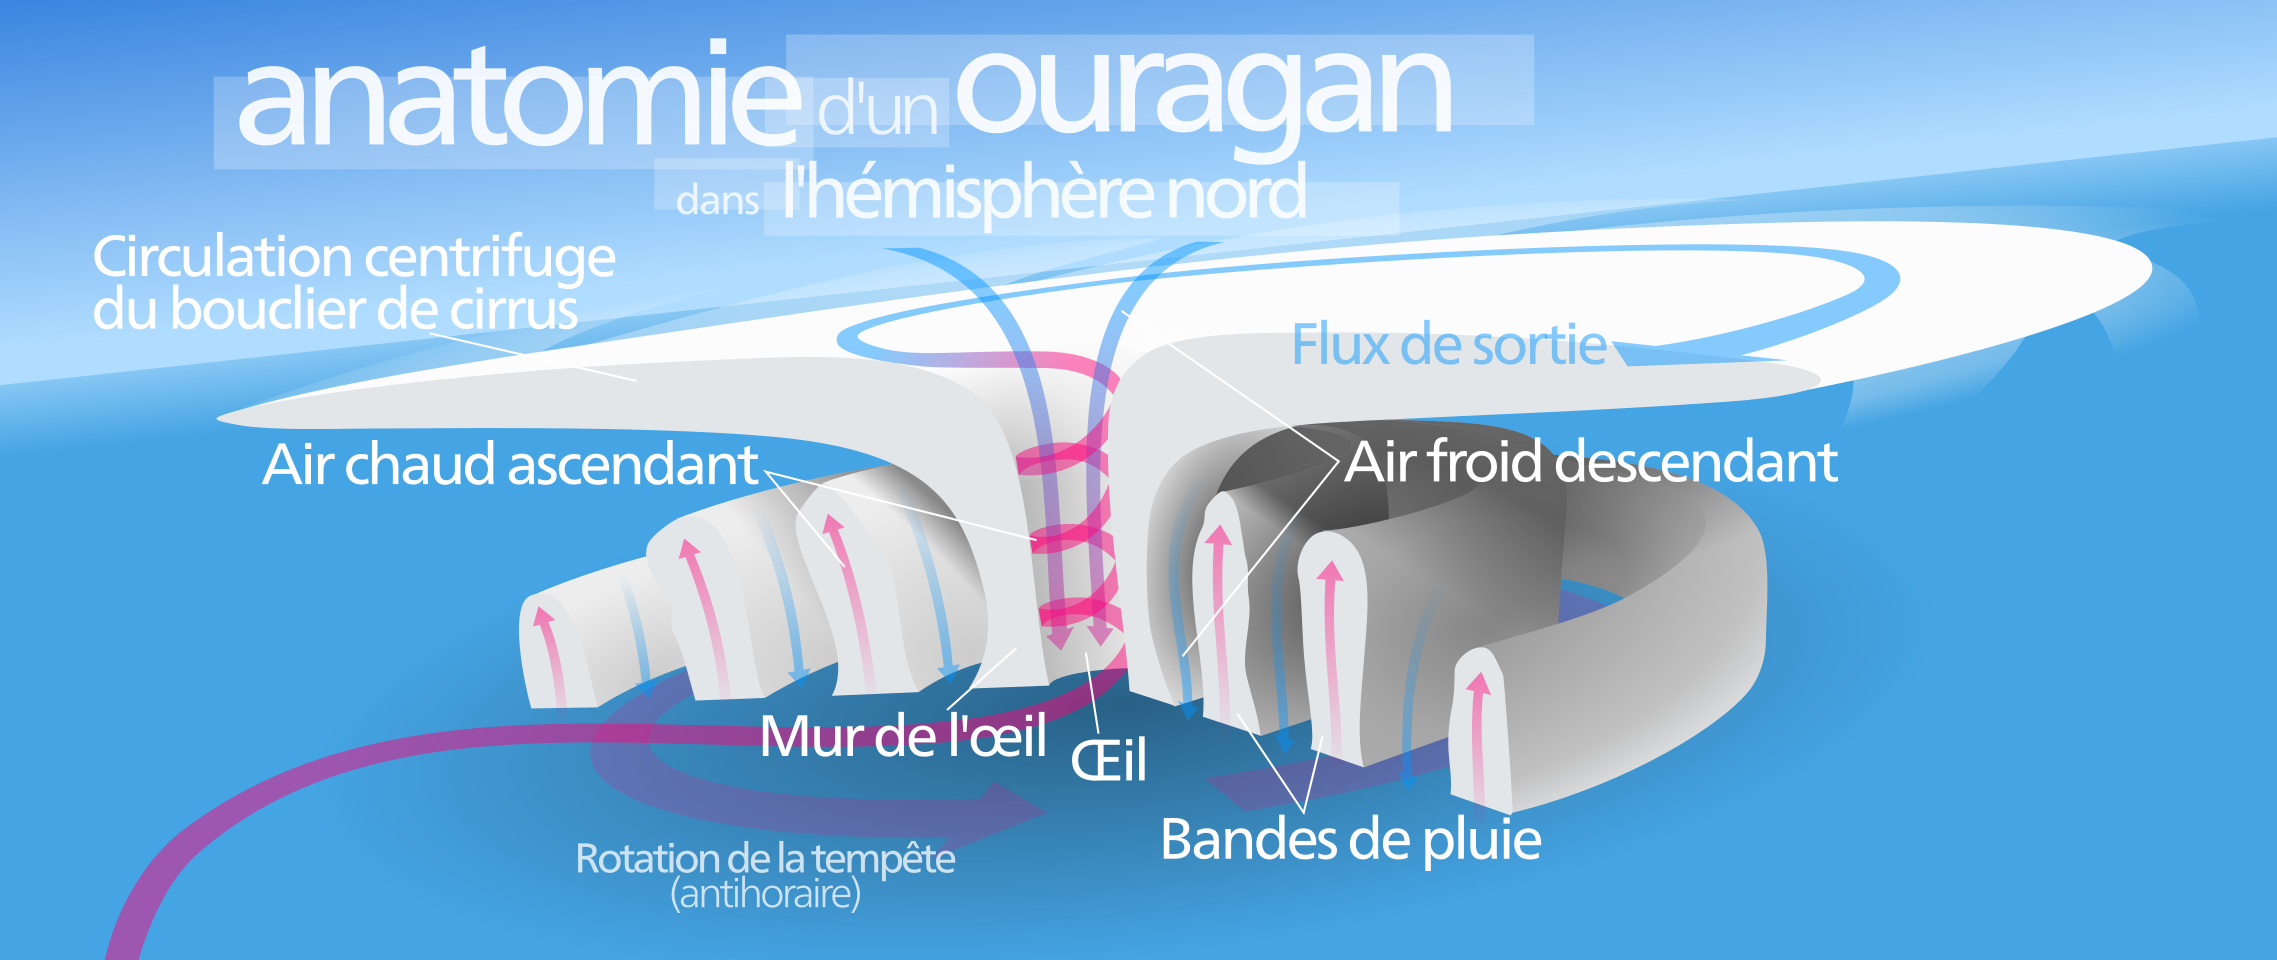
\includegraphics[width=0.9\textwidth]{Hurricane-fr.png}
    \caption{Diagramme en coupe d'un cyclone tropical, aussi appelé ouragan lorsqu'il survient dans l'océan Atlantique ou Nord-Est Pacifique -- By Kelvinsong - Own work, CC BY-SA 3.0, \url{https://commons.wikimedia.org/w/index.php?curid=23563610}}
    \label{fig:diagramme_TC}
\end{figure}

On dit que la perturbation dépressionnaire atteint le stade de cyclone tropical à proprement parler lorsque la vitesse du vent maximale à la surface et moyennée sur une certaine période, variable selon les régions du monde, atteint le seuil de \SI{33}{\metre\per\second}. En dessous de ce seuil, on parle soit de tempête tropicale si le vent maximal est supérieur à \SI{17}{\metre\per\second} ou bien de dépression tropicale si le vent maximal y est inférieur.

\subsection{Bassins d'activité et saisonnalité}\label{sec:bassins_saisons}

À l'échelle planétaire, il y a entre \numrange[range-phrase ={ et }]{82}{85} TC par an en moyenne selon les bases de données utilisées comme référence, et avec un écart-type de \num{8} TC \parencite{schreck_impact_2014}. Cette activité globale est répartie sur un total de \num{6} grands bassins océaniques. Du point de vue opérationnel, c'est à dire pour ce qui traite des aspects de surveillance et de prévision de l'activité cyclonique, ces bassins océaniques peuvent en réalité être découpés
en sous régions, dans lesquelles un centre météorologique régional spécialisé (CMRS, ou RSMC en anglais) ou un centre d'avertissements de cyclones tropicaux (TCWC -- Tropical Cyclone Warning Centres) assure ces missions. Par exemple, l'océan Sud Indien est sous la tutelle conjointe, de part et d'autre du 90\textsuperscript{ème} méridien Est, du CMRS de l'île de la Réunion (Météo-France) pour toute la partie Ouest, incluant le canal du Mozambique, tandis que la surveillance de la partie Est est assurée par les TCWC de
Perth, rattaché au Bureau of Meteorology (BoM) Australien, et de Jakarta. Néanmoins, pour la régionalisation des analyses concernant l'activité cyclonique, nous favoriserons à travers ce document les grands bassins océaniques, et utiliserons des définitions des domaines adaptées des recommandations de \cite{knutson_tropical_2020}, proposées dans un effort de standardisation afin de faciliter la comparaison entre les études sur ce sujet. Ces bassins sont présentés sur la
\cref{fig:bassins_TC}.

\begin{figure}[t]
    \centering
    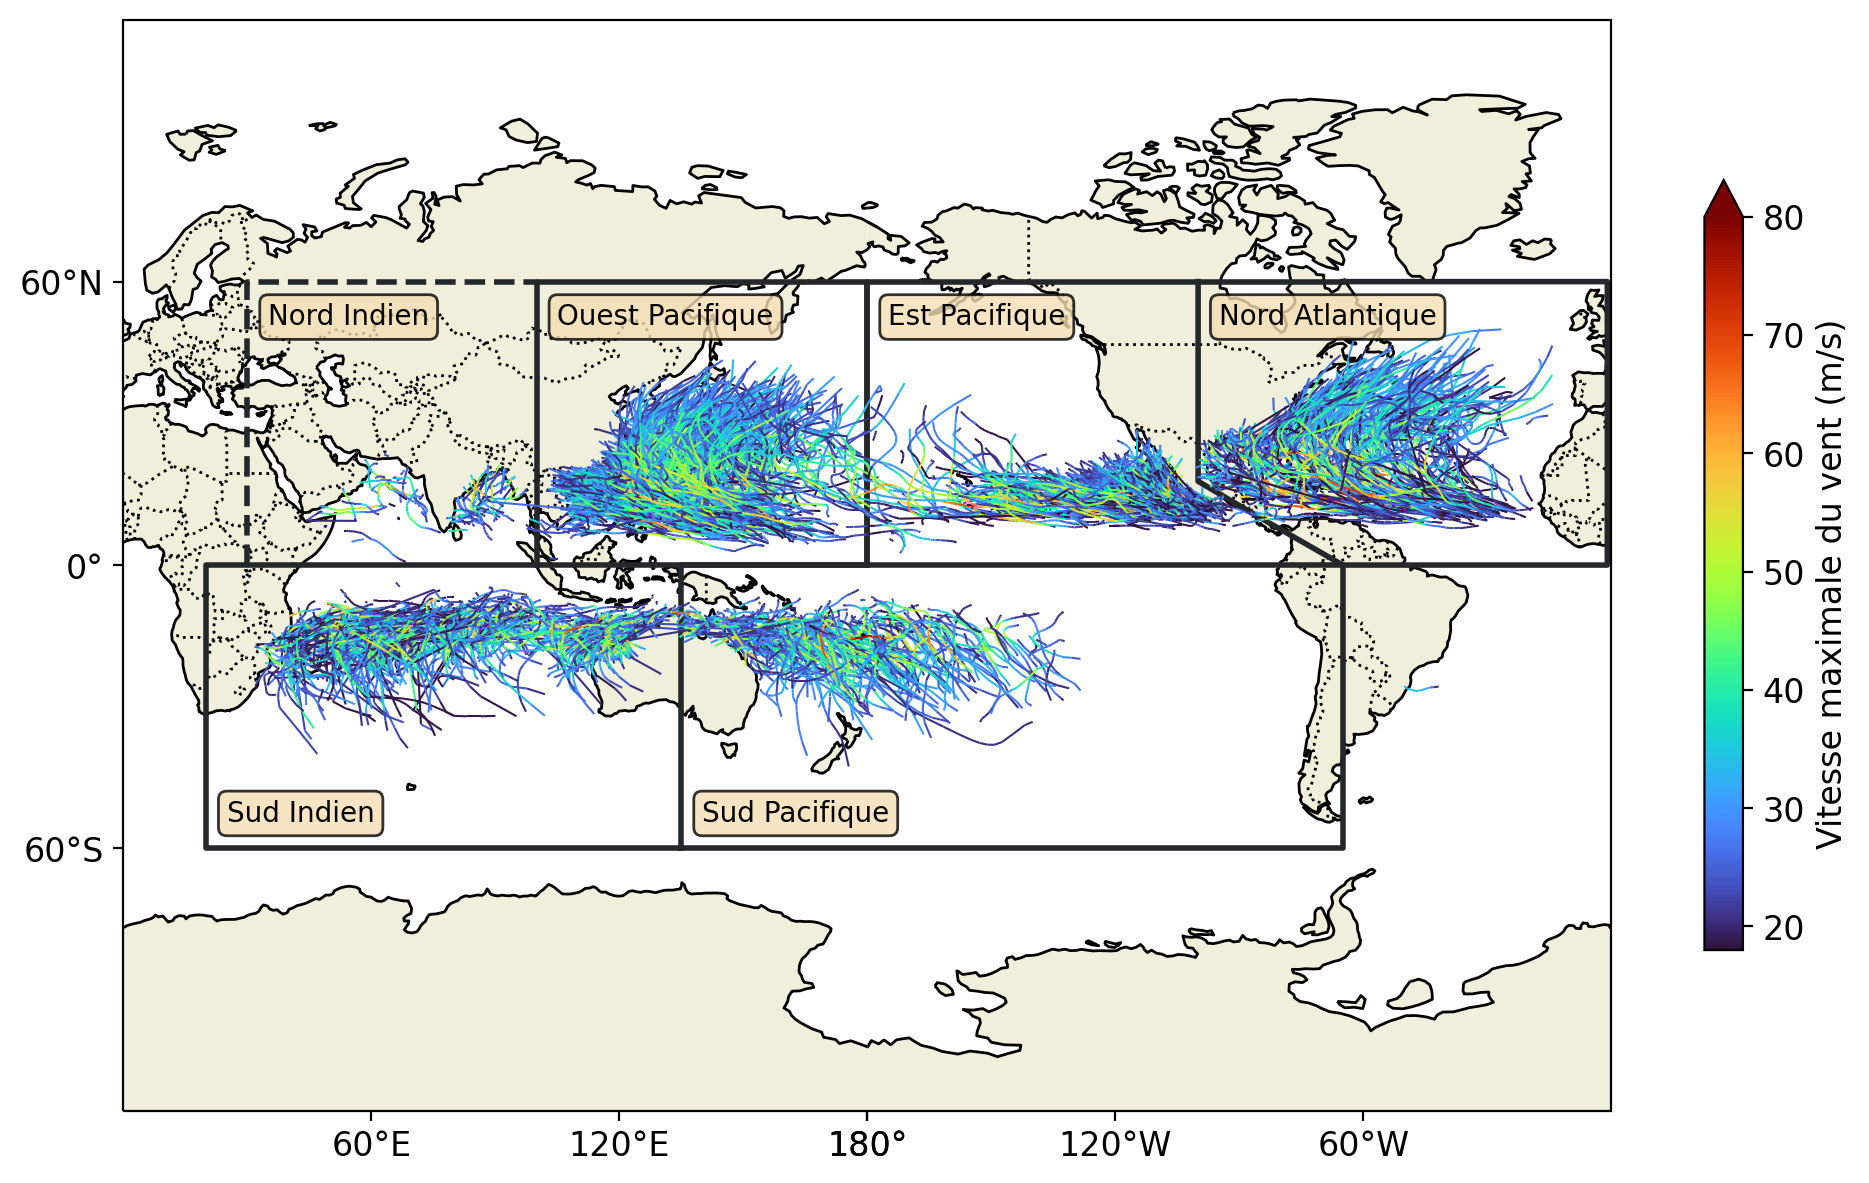
\includegraphics[width=0.9\textwidth]{Bassins_et_trajectoires.png}
    \caption{Bassins océaniques majeurs ainsi que les trajectoires des cyclones tropicaux observés entre 1981 et 2019, d'après la base de données \hbox{IBTrACS}. Les trajectoires sont colorées en fonction de l'intensité maximale des vents à chaque échéance. Les définitions des bassins océaniques utilisées ici, et plus généralement dans l'ensemble de ce document, sont issues, à quelques modifications près, des recommandations de \hbox{\cite[documents supplémentaires]{knutson_tropical_2020}}.}
    \label{fig:bassins_TC}
\end{figure}

Le bassin océanique concentrant la plus grande activité est le Ouest Pacifique (\textit{West Pacific}, WPac) avec environ \num{25} TC par an, ce qui représente environ \SI{30}{\percent} de l'activité globale. Pour les autres régions de l'hémisphère nord ; en deuxième place se trouve le bassin Est Pacifique (EPac) avec une moyenne de \num{16.5} TC par an, suivi du bassin Nord Atlantique (NAtl) avec \num{12} TC par an et enfin le bassin Nord Indien (NInd) avec entre \num{4} et \num{5} TC par
an, bassin le moins actif du monde \parencite{gray_global_1968,lander_look_1998,schreck_impact_2014}. Ce dernier se distingue également par le fait que le pays possèdent en réalité deux zones d'activité, de part et d'autre des côtes Indiennes : sur la Mer d'Arabie, à l'Ouest, et dans la Baie du Bengale, à l'Est. Au total, l'hémisphère nord contient \SI{70}{\percent} de l'activité cyclonique globale. En ce qui concerne l'hémisphère sud, ses \num{24} TC annuels en moyenne sont répartis entre l'océan indien (\textit{South Indian}, SInd) et l'océan pacifique (\textit{South Pacific}, SPac) avec une moyenne de \num{14.6} TC pour le premier et \num{9.4} TC pour le second. Il arrive parfois que des systèmes cycloniques se forment dans le sud de l'océan atlantique, bien que la région ne soit pas considérée comme
bassin cyclonique actif et qu'elle ne possède pas de CMRS. Le cas le plus notable, et l'unique système ayant atteint le seuil de vent nécessaire pour être classé comme cyclone tropical, est le cas du cyclone Catarina, en mars 2004 et ayant frappé les côtés Brésiliennes alors qu'il était au plus fort de son intensité \parencite{mctaggart-cowan_analysis_2006}. La portion de trajectoire correspondant à la partie la plus intense de ce cyclone est d'ailleurs visible sur la \cref{fig:bassins_TC}.

\begin{figure}[t]
    \centering
    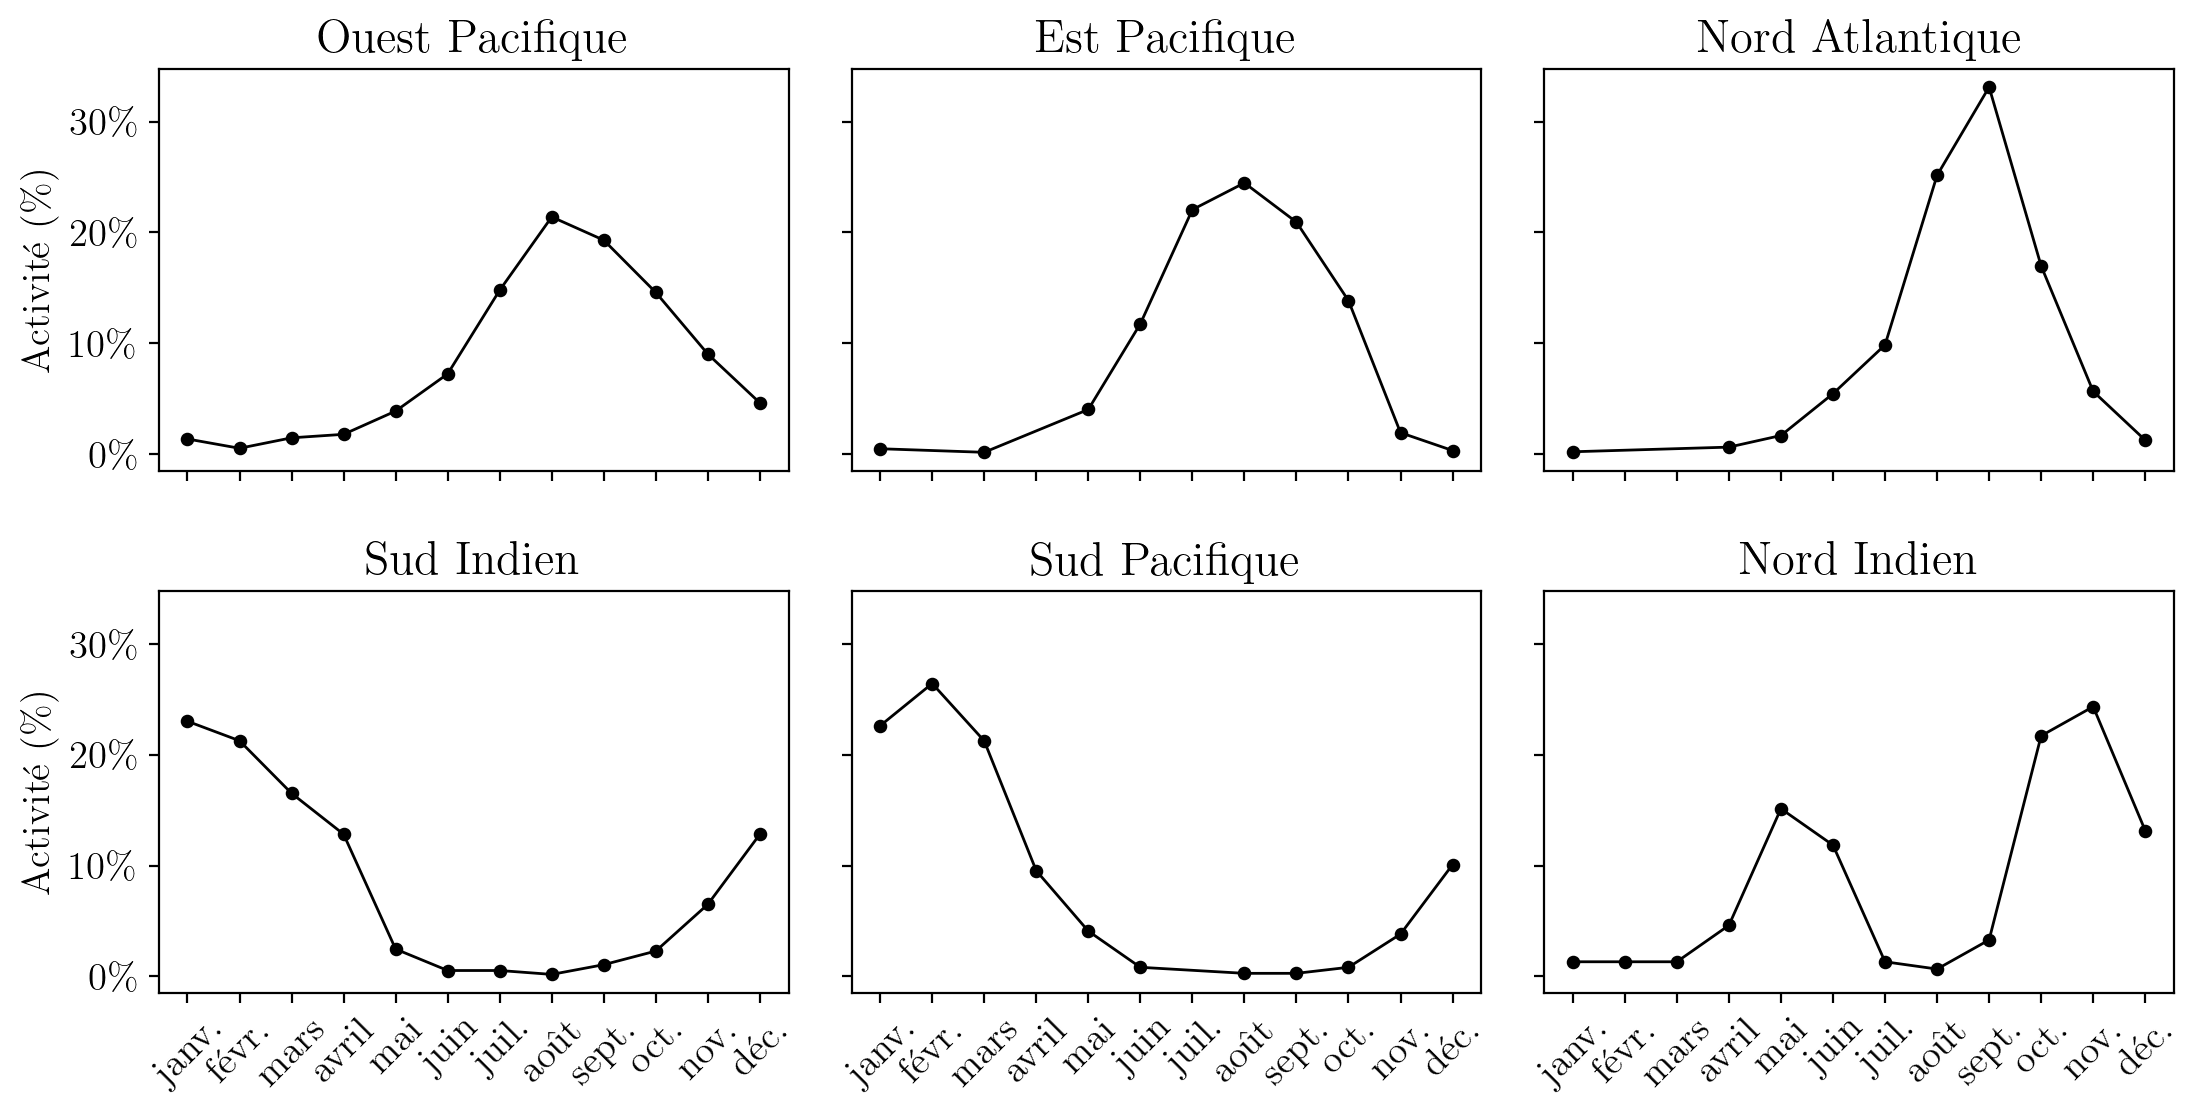
\includegraphics[width=\textwidth]{Saisons_TC.png}
    \caption{Saisonnalité de l'activité cyclonique tropicale dans les six bassins océaniques majeurs, normalisée pour chaque bassin et calculée à partir de la base de données IBTrACS entre 1981 et 2019 et en considérant pour chaque TC le mois de la première échéance où le stade de tempête tropicale est atteint.}
    \label{fig:saisons_TC}
\end{figure}

Les cyclones tropicaux surviennent principalement durant la saison chaude, avec plus ou moins d'étalement selon les régions, avec pour exception notable le cas du bassin Nord Indien. Dans l'hémisphère sud, cela signifie que l'activité cyclonique est concentrée sur les mois de novembre à avril, avec la plus grande partie située au delà de janvier, mais donc néanmoins répartie sur deux années calendaires. Pour cette raison, on considère dans l'hémisphère sud que les saisons cycloniques courent de juillet de l'année précédente à juin de
l'année courante, tandis qu'elle s'étend de janvier à décembre dans l'hémisphère nord. Le cycle saisonnier des \num{6} bassins cycloniques majeurs est présenté sur la \cref{fig:saisons_TC}. Le bassin WPac présente la plus grande dispersion, avec une activité comprise entre les mois de juin et de décembre, culminant au moins d'août. Pour l'EPac, la saison est un peu plus courte puisque, si elle commence également autour de juin, le mois de novembre ne voit quant à lui quasiment aucune activité. Le bassin NAtl présente
une activité encore plus recentrée avec un pic en septembre qui concentre un tiers de l'activité du bassin. Le bassin SInd voit sa saison débuter en novembre avec un pic en janvier, tandis que le SPac démarre un mois plus tard, en décembre, et présente un pic d'activité en février avec \SI{26}{\percent} de son activité qui est concentrée sur ce mois. Enfin, le bassin NInd se distingue ici une fois de plus puisque son cycle annuel fait apparaître deux périodes d'activité. La première, mineure,
prend place de avril à juillet, tandis que la seconde, plus importante, a lieu de septembre à janvier. Cette coupure dans le cycle annuel s'explique par le phénomène de mousson indienne, qui a lieu durant l'été, et qui apporte du cisaillement vertical dans l'atmosphère, élément défavorable à la cyclogénèse \parencite{gray_global_1968}, comme développé dans la \cref{sec:conditions_cyclogenese}.

\subsection{Risques associés et enjeux}

Les cyclones tropicaux constituent les évènements météorologiques les plus extrêmes, les plus destructeurs et aussi les plus dangereux pour les populations. D'après l'étude de \cite{doocy_human_2013}, le nombre médian de victimes par TC s'élève à \num{14} vies (\num{430} en moyenne), pour un bilan humain total estimé entre les années 1980 et 2009 à \num{412644} morts et \num{290654} blessés. Les deux tiers de ce nombre sont attribués à seulement deux évènements : Le cyclone Gorky de 1991 ayant fait \num{138866} victimes au Bangladesh, et le cyclone Nargis en 2008, en
Birmanie, avec \num{138366} victimes. Outre les morts, le nombre total de personnes affectées d'une façon ou d'une autre par les TC est estimé à plus de \num{466} millions, ce qui inclut \num{20} millions de personnes qui se sont retrouvées sans abri. Ainsi, la région de l'Asie du Sud-est, telle que définie par l'Organisation Mondiale de la Santé, concentre \SI{80}{\percent} des décès causés par les cyclones tropicaux, et \SI{53}{\percent} de la population affectée, tandis qu'elle ne
concentre que \SI{9}{\percent} des évènements impactant, ce qui montre alors que les plus forts impacts sont causés par quelques évènements extrêmes.

Pour ce qui est du coût des dégâts matériels associés aux TC, ils sont difficiles à estimer à l'échelle globale car ils n'ont étés rapportés que dans \SI{15.4}{\percent} des cas, toujours d'après \cite{doocy_human_2013}. Ces coûts sont néanmoins d'autant plus importants que les pays concernés sont riches et dotés d'infrastructures coûteuses. Le Centre National d'Information sur l'Environnement (NCEI) de l'Agence Américaine d'Observation Océanique et Atmosphérique (NOAA) recense tous les
évènements météorologiques extrêmes impactant les États-Unis dont les coûts dépassent le seuil de \num{1}~milliard de dollars. Ainsi, entre 1980 et 2020, les dégâts causés par les cyclones tropicaux sont évalués, en tenant compte de l'inflation, à \num{1145.3}~milliards de dollars, ce qui concentre \SI{52.3}{\percent} du coût total causé par l'ensemble des extrêmes météorologiques considérés ---~loin devant la deuxième plus importante cause de dégâts matériels, à savoir les fortes tempêtes, qui
concentrent \SI{15}{\percent} des coûts totaux~--- et ce qui représente un coût moyen de \num{21.6}~milliard de dollars par évènement
\parencite{smith_billiondollar_2020}.

Les risques associés aux TC sont nombreux et divers : Vents extrêmes, fortes précipitations et inondations, orages, tornades et glissements de terrain. Mais le plus grand risque provient des ondes de marées. Sous l'effet conjugué des vents et de la pression centrale du cyclone, le niveau de la mer augmente fortement et rapidement, et se retrouve poussé vers l'intérieur des terres, parfois sur
plusieurs dizaines de kilomètres. Les ondes de marées
sont le danger principal associé aux TC et aussi la première cause de mortalité durant ces évènements \parencite{needham_review_2015}. Si chacun de ces risques peut, lorsque pris individuellement, causer des pertes considérables, matérielles comme immatérielles, le danger est d'autant plus grand lorsque ces aléas surviennent simultanément et interagissent entre eux, avec des impacts pouvant perdurer longtemps après le passage du cyclone. En effet, suite au passage d'un cyclone tropical, il n'est pas rare de voir l'émergence de maladies infectieuses, en
particulier dans les pays en voie de développement \parencite{shultz_epidemiology_2005}. Cette émergence se voit en effet favorisée, entre autres, par la perturbation des infrastructures de santé publique ---~incluant les hôpitaux et les centres de soins, mais également les réseaux de distribution en eau potable~--- mais aussi par les regroupements des populations dans des refuges surpeuplés, et plus généralement par une plus grande exposition de ces derniers à l'environnement suite aux dommages causés aux
habitations. Il en ressort donc que les dégâts matériels et économiques causés par les cyclones tropicaux peuvent également avoir un coût en vies humaines.

Le plus un cyclone tropical est grand et développé, le plus les risques sont accrus. Bien qu'il soit difficile de déterminer précisément la relation liant d'une part l'intensité d'un cyclone et les dégâts associés d'autre part, il est néanmoins admis que le potentiel de destruction d'un cyclone dépend au moins de l'intensité de ses vents. Une métrique classiquement utilisée pour quantifier l'activité cyclonique sur une saison donnée consiste par exemple à faire la somme des vents
maximums soutenus, élevés au carré, avec une période de six heures, sur l'ensemble des systèmes de la saison lorsqu'ils dépassent au moins le stade de tempête tropicale~--- métrique appelée l'énergie cumulative des cyclones tropicaux (\textit{Accumulated Cyclone Energy}, ACE, \cite{bell_climate_2000}). Si d'autres métriques sont parfois utilisées et jugées plus pertinentes pour évaluer le potentiel destructeur d'un TC, elles restent toutefois basées sur la vitesse du vent
\parencite{powell_tropical_2007}. Ainsi, en supposant que le risque cyclonique demeure constant dans un climat plus chaud et que les pays concernés par ce risque continuent à se développer, alors les dégâts économiques ne peuvent
qu'augmenter. Sous cette hypothèse de stationnarité, les travaux de \cite{ye_dependence_2020} suggèrent qu'un doublement de la valeur des actifs exposés à ce risque en Chine pourrait engendrer une hausse de \SI{80}{\percent} des dégâts économiques induits par les TC. Or, rien ne permet d'affirmer la validité de cette hypothèse, étant données les incertitudes associées aux projections futures de l'activité cyclonique tropicale (voir \cref{sec:projections_futures}). Par conséquent,
l'évolution de l'activité cyclonique dans un contexte de réchauffement global, en particulier pour ce qui concerne les questions d'intensité et de fréquence des TC, constitue un enjeu de première importance.

%-------------------------------------------------------------------------------
\section{Ingrédients de la cyclogénèse}
  
\subsection{Conditions de formation}\label{sec:conditions_cyclogenese}

On appelle \textquote{cyclogénèse} le processus par lequel un cyclone tropical se développe et s'intensifie. Bien que les mécanismes précis permettant d'expliquer ce processus ne soient pas encore compris, malgré des décennies d'efforts consacrés à cette question \parencite{yanai_formation_1964, montgomery_tropical_1993, gray_formation_1998, tory_tropical_2010}, il existe néanmoins un consensus quant aux facteurs qui y sont favorables. Les travaux de \cite{gray_global_1968}, complétés dans
\cite{gray_tropical_1975}, consistuent, à partir des observations disponibles à l'époque, une étude globale sur l'origine des cyclones tropicaux et font référence en la matière. Six facteurs sont ainsi identifiés et brièvement présentés ci-dessous.

\subsubsection{Vorticité relative en basses couches}

Les cyclones tropicaux se forment toujours à partir de perturbations atmosphériques préexistantes. Ce sont souvent des petits systèmes dépressionnaires provenant de la zone de convergence intertropicale (ZCIT) \parencite{gray_global_1968}, ou encore des ondes d'est tropicales, comme dans le cas de l'océan Atlantique où ces ondes peuvent jouent le rôle de précurseurs \parencite{thorncroft_african_2001,patricola_response_2018}. Ces perturbations apportent une
vorticité initiale, ou tourbillon, qui, par convergence frictionnelle, apporte de la vapeur d'eau provenant de la mer vers le cœur du système, au niveau de la couche limite atmosphérique. Cette vapeur est entrainée en altitude par mouvement convectif, puis condensée, libérant de ce fait de la chaleur latente en haute troposphère, contribuant ainsi à entretenir le fonctionnement du cyclone. Ce mécanisme constitue la source principale d'énergie des cyclones tropicaux \parencite{emanuel_dependence_1987}.

\subsubsection{Rotation de la Terre}

La rotation de la Terre induit, du point de vue d'un observateur appartenant au même référentiel, une force sur tous les objets se déplaçant à la surface de la planète et appelée force de Coriolis. Cette force, qualifiée d'inertielle ou de fictionnelle, en ce sens qu'elle n'est le résultat que du fait que le référentiel d'observation est non inertiel, dévie les objets perpendiculairement à la direction de leur mouvement, vers la gauche si le référentiel tourne dans le sens horaire et vers la droite si le référentiel possède une rotation anti-horaire. Dans le cas
des cyclones tropicaux, la force de Coriolis tend à dévier les cyclones vers les pôles géographiques (voir \cref{fig:bassins_TC}).

Mais outre l'effet sur leur trajectoires, la rotation de la Terre joue également un rôle primordial dans la circulation cyclonique, puisque c'est cette force est à l'origine même du mouvement de rotation dans la circulation cyclonique. Cette force varie avec le sinus de la latitude et est donc nulle à l'équateur. À proximité de l'équateur, la force de Coriolis est donc négligeable et les vents de la couche limite atmosphérique ne sauraient se maintenir au delà de quelques mètres par secondes
\parencite{gray_tropical_1975}. La force de Coriolis permet au vortex d'atteindre l'équilibre du vent gradient, mentionné dans la \cref{sec:quest_ce_qu_un_cyclone} et donc de se développer jusqu'à devenir un cyclone tropical. Par conséquent, la cyclogénèse ne peut pas se produire à l'équateur, et il est généralement admis qu'une distance à l'équateur de \num{4}~à~\ang{5} est requise pour qu'un cyclone tropical puisse se développer.

\subsubsection{Faible cisaillement vertical du vent}

Le cisaillement du vent, ou plus précisément ici, le cisaillement vertical du vent horizontal, exprime la manière dont le vent horizontal varie avec l'altitude, en intensité comme en direction. Dans le cas des cyclones tropicaux, on le mesure (ou le calcule) sur toute la hauteur de la troposphère, c'est à dire entre la tropopause à \SI{200}{\hecto\pascal} et la basse troposphère, typiquement à \SI{850}{\hecto\pascal}. Le cisaillement détermine donc dans quelle mesure le réchauffement des
couches supérieures de la troposphère sont ventilées à l'écart de la perturbation, et limite donc la capacité du système à accumuler de la chaleur en son cœur \parencite{gray_tropical_1975}. Le cisaillement vertical est donc très défavorable à la cyclogénèse, et il est admis que cette dernière ne peut avoir lieu si le cisaillement est supérieur à \SI{10}{\metre\per\second}.

\subsubsection{Température de surface de la mer}

Un cyclone tropical consomme environ \SI{15}{\mega\joule} par jour de chaleur sensible et latente extraite de la surface océanique \parencite{gray_tropical_1975}. De plus, la circulation cyclonique produit une remontée d'eau océanique (upwelling) autour du centre du système. Pour ces raisons, la cyclogénèse nécessite non seulement que la température de surface océanique (\textit{sea surface temperature}, SST) dépasse un certain seuil ---~évalué à \SI{26}{\degreeCelsius}, sinon quoi la
flottabilité n'est pas suffisante pour assurer la convection~--- mais également que cette température soit atteinte sur au moins \SI{60}{\metre} de profondeur d'eau. En effet, si ce seuil de SST n'est atteint qu'en surface, le phénomène d'upwelling apportera de l'eau plus froide qui ne permettra plus d'alimenter le système. Ce besoin important en chaleur a généralement pour conséquence la désintensification rapide du TC mature lorsqu'il atteint les terres.

\subsubsection{Humidité relative et instabilité atmosphérique}

Ces deux derniers facteurs que sont l'humidité relative en moyenne troposphère, c'est à dire autour de \SI{600}{\hecto\pascal}, et la notion de stabilité atmosphérique, sont, dans le cadre de la cyclogénèse, étroitement liés. La stabilité de l'atmosphère, à fortiori lorsqu'elle est chargée en vapeur d'eau, dépend du gradient vertical de température potentielle équivalente, notée $\theta_e$ et définie comme la température que la parcelle d'air atteindrait si tout son contenu en vapeur d'eau
venait à condenser et qu'elle était ramenée au niveau du sol de manière adiabatique. Le processus de convection des cumulonimbus, à l'origine de la formation d'un cyclone tropical, nécessite en effet une forte diminution de $\theta_e$ entre la couche limite atmosphérique et la moyenne troposphère, c'est à dire une atmosphère instable. Par ailleurs, la convection profonde est favorisée par une atmosphère à haute humidité relative en moyenne troposphère, car à température égale, une
parcelle d'air humide possède une plus grande flottabilité qu'une parcelle d'air sec. Enfin, toujours d'après \cite{gray_tropical_1975}, une humidité relative élevée en haute troposphère favorise les précipitations et donc la libération d'enthalpie qui vient renforcer le cœur chaud du système.

\subsection{Modèles conceptuels de fonctionnement}

\subsubsection{CISK}

\cite{charney_growth_1964,ooyama_dynamical_1964,ooyama_numerical_1969}

\subsubsection{WISHE}

\cite{emanuel_airsea_1986,emanuel_largescale_1994}

%-------------------------------------------------------------------------------
\section{Cyclones tropicaux et changement climatique}

\subsection{Bases de données observationelles}

Un pré-requis pour pouvoir traiter de changement climatique, quelque soit l'objet d'étude, est de disposer de données observationelles le plus fiables possibles, et sur la plus longue période possible. Les climatologies sont en effet basées sur des périodes d'au moins \num{30} ans. Un des problèmes fondamentaux avec les réseaux d'observation météorologiques en général, est que les instruments s'améliorent avec le temps, les réseaux s'étendent et se densifient, ce qui donne lieu à
des fortes hétérogénéités et ruptures temporelles dans la qualité des données. L'observation des cyclones tropicaux ne fait pas exception à cette règle. Les cyclones étant des phénomènes prenant place sur mer, les premiers relevés météorologiques de cyclones tropicaux étaient réalisés par les marins et consignés dans leurs journaux de bords \parencite{knapp_international_2010}. Avec le temps, et étant donnée le fort potentiel d'impact de ces systèmes, les sources d'observations se sont
multipliées et diversifiées, de manière très inégale selon les régions. Les États-Unis déploient par exemple des avions de reconnaissances dédiés à la recherche et à l'observation des cyclones tropicaux au large des côtes atlantiques depuis \num{1946}, bassin océanique qui est encore à ce jour le seul à bénéficier de ce type d'observations de manière régulière. D'autres sources d'observations incluent notamment les stations météorologiques terrestres, bouées instrumentalisées, radars et
enfin radio
sondages, ces derniers pouvant être réalisés par largage aérien directement dans le cyclone. Néanmoins, la véritable rupture technologique eut lieu avec l'ère satellitaire, réellement entérinée à la fin des années 70. L'observation par satellite permet d'une part de détecter la quasi totalité des cyclones, mais aussi d'estimer systématiquement leur intensité, même en l'absence de mesures \textit{in situ}, par analyse de Dvorak consistant en
une estimation indirecte et partiellement subjective de l'intensité à partir de la structure des amas nuageux et de leur température \parencite{dvorak_tropical_1975,velden_development_1998,olander_development_2002,olander_advanced_2007,olander_advanced_2019}\footnote{Le perfectionnement de la méthode de Dvorak originelle avec le temps est indicatif du fait que les données observées relatives à l'intensité des cyclones tropicaux souffrent d'hétérogénéité temporelle, et ce même après le début de l'ère
satellitaire.}. En effet, un bon nombre de systèmes qui n'atteignaient jamais les côtes
passaient inaperçus avant cela \parencite{landsea_atlantic_2004}, et un grand nombre de cyclones observés avant ce tournant contiennent des données manquantes. Pour ces raisons,
et bien qu'il soit possible d'obtenir des données locales relatives aux cyclones tropicaux remontant jusqu'en \num{1850}, nous nous limiterons dans l'ensemble de ce document à utiliser des données issues d'observations réalisées à partir de \num{1980}.

La constitution de bases de données cycloniques passe par la mise au point, pour chaque système, de ce qui est nommé la \textit{best track}. Il s'agit de la meilleure estimation, réalisée à posteriori, de la position et de l'intensité du cyclone, et ce à partir de l'ensemble des sources d'information disponibles. Il en résulte que la best track ne représente pas nécessairement le cycle de vie réel du cyclone, mais plutôt une version artificiellement lissée, aussi bien du point de vue de sa trajectoire,
que de ses variations en intensité et en taille, et ce même si le système a été observé avec une grande précision en premier lieu \parencite{landsea_atlantic_2013}. Il est important de souligner qu'il n'existe pas de méthodologie unifiée à l'échelle globale sur la manière d'établir les best tracks. Comme mentionné à la \cref{sec:bassins_saisons}, les zones d'activité sont sous la supervision d'un CMRS ou d'un TCWC ---~eux-mêmes sous la tutelle de l'Organisation Météorologique Mondiale (\textit{World
Meteorological Organization}, WMO)~--- lesquels établissent les best tracks pour leur secteur, selon des procédures opérationnelles qui leur sont propres, donnant lieu à une forte hétérogénéité spatiale \parencite{schreck_impact_2014}. L'estimation de l'intensité du vent est probablement le cas le plus probant pour mettre en évidence la difficulté à unifier toutes ces données. En effet, outre le fait qu'un cyclone tropical peut être observé par plus ou moins de moyens différents ---~chaque outil fournissant des données plus ou moins fiables~--- et outre aussi la
subjectivité inhérente à l'analyse, tous les CMRS
n'utilisent pas le même temps d'intégration pour la mesure du vent maximum soutenu (\textit{Maximum Sustained Wind}, MSW). Le WMO définit le MSW comme le vent maximal mesuré \SI{10}{\meter} au dessus de la surface et soutenu pendant \num{10} minutes. Or, certains centres intègrent le vent sur \num{1} minute, et d'autres sur \num{3} minutes. Par ailleurs, comme le souligne \cite{knapp_international_2010}, un coefficient de conversion de \num{0.88} est parfois utilisé
par les CMRS eux-mêmes pour convertir un vent sur \num{1} minute en un vent sur \num{10} minutes, tandis que le WMO recommande d'utiliser la valeur de \num{0.93}. Ainsi, les différences dans la façon dont chaque CMRS analyse les cyclones tropicaux compliquent non seulement la comparaison des données issues de différents bassins océaniques, mais elles constituent aussi une source d'incertitude supplémentaire pour la comparaison entre les études traitant de l'activité cyclonique globale, puisque toutes ne procèdent pas de la même
façon pour tenter de les harmoniser.

En dépit de toutes ces limitations, la mise en commun des données issues de chaque centre spécialisé en un fichier unique est précisément l'objectif de la base de données IBTrACS (\textit{International Best Track Archive for Climate Stewardship}, \cite{knapp_international_2010}). Bien qu'IBTrACS puisse être moins détaillé que certaines bases de données locales, comme par exemple HURDAT2 pour l'océan Atlantique \parencite{landsea_atlantic_2013} qui fournit une information sur la taille des
cyclones à travers
l'étendue maximale des vents à \num{34}, \num{50} et \SI{64}{\knot} dans les quatre quadrants autour du centre du système, elle possède donc néanmoins la qualité de couvrir tous les bassins géographiques et fournit également une grande quantité de méta données permettant de filtrer au mieux les informations. Pour cette raison, IBTrACS est la base de données observationelle qui est utilisée à travers tout ce document, comme c'est déjà le cas pour les
\cref{fig:bassins_TC,fig:saisons_TC}.

\subsection{Les modèles de climat}



\subsection{Les cyclones dans les modèles de climat}

\cite{manabe_tropical_1970}

\subsection{Consensus actuel sur les projections futures}\label{sec:projections_futures}

\cite{seneviratne_weather_2021}

\subsection{Détection objective v.s indices de cyclogénèse}

%-------------------------------------------------------------------------------
\section{Synthèse}

\end{document}
